\documentclass[11pt,titlepage,fleqn]{article}

\usepackage{amsmath}
\usepackage{amssymb}
\usepackage{latexsym}
\usepackage[round]{natbib}
\usepackage{xspace}
\usepackage{graphicx}
\usepackage{epstopdf}
%\usepackage{epsfig}

\usepackage{pifont}   % search for \ding

%\usepackage{fancyhdr}
%\pagestyle{fancy}

%=====================================================
%       SPACING COMMANDS (Latex Companion, p. 52)
%=====================================================

\usepackage{setspace}

%---------------------------
\newcommand{\matlab}{\textsc{Matlab}\xspace}
%---------------------------
\renewcommand{\baselinestretch}{1.0}

\textwidth 460pt
\textheight 700pt
\oddsidemargin 0pt
\evensidemargin 0pt

% see Latex Companion, p. 85
\voffset     -50pt
\topmargin     0pt
\headsep      20pt
\headheight    0pt
\footskip     30pt
\hoffset       0pt

\include{carlcommands}
%\input{dp_header}

\graphicspath{
  {/home/vipul/REPOSITORIES/IITR_seismo/classes/ES510/latex/figures/}
  }

\begin{document}

\noindent Course: Numerical Methods and Computer Programming\\
\noindent Code: ES 510\\
\noindent Instructor: Vipul Silwal (\verb+vsilwalfes@iitr.ac.in+) \\ 
\noindent Last Compiled: \today \\

{\huge Taylor Series and Fourier Series}

\tableofcontents
%% ------------------------------------------------------------------------ %%
\begin{section}{Taylor Series}
by Brook Taylor (1685-1731) - English mathematician.

Taylor series is a representation of a function as a sum of its derivates: 

\begin{equation}
f(x+h) = f(x) + hf'(x) + \frac{h^2}{2!}f''(x) + \cdots + \infty 
\end{equation}
And after approximating to n-th degree
\begin{equation}
f(x+h) = f(x) + hf'(x) + \frac{h^2}{2!}f''(x) + \cdots +  \frac{h^{n-1}}{(n-1)!}f^{n-1}(x) + \frac{h^n}{n!}f^n(x + \lambda h)
\end{equation}
where $\lambda \in [-0,1]$ gives the error term.

The benefit of replacing a function with its polynomial is that its generally easier to work with polynomials (integrate, etc).

{\bf Example:}
\begin{eqnarray*}
f(x) &=& \log(1 + x) \\
f'(x) &=& \frac{1}{(1 + x)} \\
f''(x) &=& \frac{-1}{(1 + x)^2} \\
f'''(x) &=& \frac{2}{(1 + x)^3} \\
f''''(x) &=& \frac{-2 \cdot 3}{(1 + x)^4} \\
\end{eqnarray*}
Expanding the series near $x=0$ (called Maclaurin's series), we get:

\begin{equation*}
\log(1+x) = x - \frac{x^2}{2} + \frac{x^3}{3} - \frac{x^4}{4} + \cdots
\end{equation*}

\begin{subsection}{Applications}
{\bf Newton's method}: \\
Is an iterative method of finding the root of a function $f(x)$ where we start with some initial guess $x_0$ and successively iterate until we get a sufficient precise solution:
\begin{eqnarray}
x_1 &=& x_0 - \frac{f(x_0)}{f'x_1)} \\
\vdots \\
x_{n+1} &=&  x_n-\frac{f(x_n)}{f'x_n)}
\end{eqnarray}
(provided the initial guess is close to the root). 

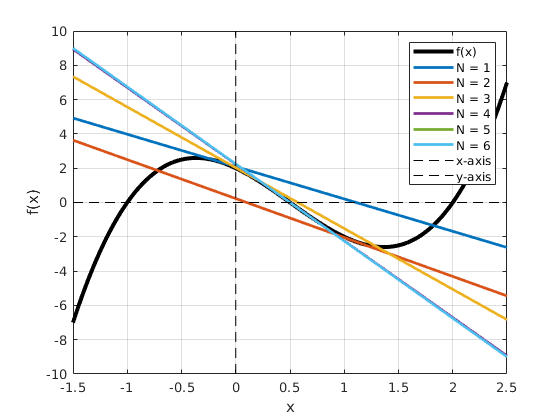
\includegraphics[scale=0.75]{newtons_method.png}

{\bf Computing gradient:}
\begin{equation}
\frac{f(x+h) - f(x)}{h} = f'(x) + \frac{h}{2} f''(x) + \cdots + \frac{(x+h-\xi)^k}{k!} \frac{f^k (x+h-\xi)}{h}
\end{equation}
(we will see more applications of this in lecture on Simpson's rule)\\
%XXX Add mid-point example

{\bf Multi-variate case:}

Specialized case of Newton's method can be used to solve for non-linear inverse problems. In this section we will assume $\bx$ is a vector (in geophysical modeling this would be {\it model parameters}).
\begin{equation}
f(\bx_0 + \Delta \bx) \approx f(\bx_0) + \nabla f(\bx_0) \Delta \bx + \frac{1}{2} \Delta \bx^T \bH(f(\bx_0)) \Delta \bx 
\end{equation}

where $\nabla f(\bx_0)$ is the gradient (or Laplacian of $f(\bx)$):
\begin{equation}
\nabla f(\bx_0) = 
\begin{bmatrix} 
\frac{\delta f(\bx)}{\delta x_1}\\
\vdots \\
\frac{\delta f(\bx)}{\delta x_n}\\
\end{bmatrix} _{\bx = \bx_0}
\end{equation}

and $\bH(f(\bx_0))$ is the Hessian
\begin{equation}
\bH(f(\bx_0)) = 
\begin{bmatrix} 
\frac{\delta^2 f(\bx)}{\delta x_1^2} \cdots \frac{\delta^2 f(\bx)}{\delta x_1 x_n}\\
\vdots \ddots \vdots \\
\frac{\delta^2 f(\bx)}{\delta x_n x_1} \cdots \frac{\delta^2 f(\bx)}{\delta x_n^2}\\
\end{bmatrix} _{\bx = \bx_0}
\end{equation}

For non-linear problems $f(\bx)$ would generally be:
\begin{equation}
f(\bx) = \sum_{i=1}^n \left ( \frac{G(\bem)_i - d_i}{\sigma_i} \right )^2
\end{equation}

\end{subsection}

\end{section}

\begin{section}{Fourier Series}
Is a way of representing a {\it periodic} function $f(x)$ as a weighted sum of sines and cosines.

\begin{equation}
f(x) = a_0 + \sum_{n=1}^{\infty } (a_n \cos(nx) + b_n \sin(nx))
\end{equation}
where $a_0, a_n,$ and $b_n$ are for a $2\pi$ periodic function which is integrable in $[-\pi, \pi]$:
\begin{eqnarray}
a_0 &=& \frac{1}{2\pi} \int_{-\pi}^\pi f(x) dx\\
a_n &=& \frac{1}{\pi} \int_{-\pi}^\pi f(x) \cos(nx) dx\\
b_n &=& \frac{1}{\pi} \int_{-\pi}^\pi f(x) \sin(nx) dx \label{fourier}
\end{eqnarray}

{\bf Example:}
(\verb+Also see lab's MATLAB example+)

Consider a function
\begin{equation*}
f(x) = x, \pi \leq x \leq \pi
\end{equation*}
\begin{eqnarray*}
a_0 &=& \frac{1}{2\pi} \int_{-\pi}^\pi x dx\\
&=& 0\\
a_n &=& \frac{1}{\pi} \int_{-\pi}^\pi x \cos(nx) dx\\
&=& 0\\
b_n &=& \frac{1}{\pi} \int_{-\pi}^\pi x \sin(nx) dx\\
&=& \frac{1}{pi} \left [ -\frac{x \cos(nx)}{n} + \frac{\sin(nx)}{n^2} \right ]_{-\pi}^\pi \\
&=& -\frac{2}{n} \cos(n\pi)\\
&=& \frac{2}{n} (-1)^{n+1}
\end{eqnarray*}

Hence, $f(x)$ can be approximated by:
\begin{equation*}
f(x) \sim 2 \left ( \sin(x) - \frac{\sin(2x)}{2} + \frac{\sin(3x)}{3} + \cdots \right)
\end{equation*}
\end{section}

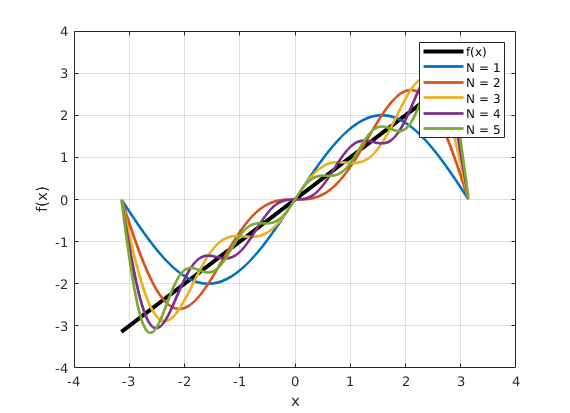
\includegraphics[scale=0.75]{fourier_x.png}

{\bf Note: }
If $f(x)$ is integrable in $[-L, L]$ substitute $t = \frac{Lx}{\pi}$. This ends up giving:
\begin{eqnarray}
a_0 &=& \frac{1}{2L} \int_{-L}^L f(x) dx\\ 
a_n &=& \frac{1}{L} \int_{-L}^L f(x) \cos(n\frac{\pi x}{L}) dx\\ 
b_n &=& \frac{1}{L} \int_{-L}^L f(x) \sin(n\frac{\pi x}{L}) dx \label{fourier_gen}
\end{eqnarray}

%----------------------------------------------
\begin{section}{Exercise}
\begin{enumerate}
\item Compute taylor series expansion for: $\sin x, \cos x$ upto third degree for $x = \pi/3$ and compare with the actual values.

\item Compute the fourier series expansion for a box car function:
\begin{equation}
f(x) = \begin{cases}
0, \pi \leq x \leq 0\\
\pi , 0 \leq x \leq \pi
\end{cases}
\end{equation}

\item Show how to get equation 15-\ref{fourier_gen} after substituting $t = \frac{Lx}{\pi}$ in equation 12-\ref{fourier}.

\item Show that fourier series terms form an orthonormal basis.

\end{enumerate}

\end{section}

\end{document}
